\documentclass{resume}

\begin{document}

\fontfamily{ppl}\selectfont

\noindent
\begin{tabularx}{\linewidth}{@{}m{0.8\textwidth} m{0.2\textwidth}@{}}
{
    \textcolor{ceruleanblue}{\Large{Anna Fedorova}} \newline
    \textcolor{ceruleanblue}{\small\textbf{Software Engineer}} \newline
    \small{
        \clink{
            \href{mailto:anna.fedorova.se@gmail.com}{anna.fedorova.se@gmail.com},
            {\fontdimen2\font=0.75ex +49 1520 7153706}
        } \newline
        Neufriedenheimer Platz 8, 81375, Munich, Germany \newline
        Github profile: \href{https://github.com/Fedannie}{https://github.com/Fedannie}
    }
} & 
{
    %\hfill
    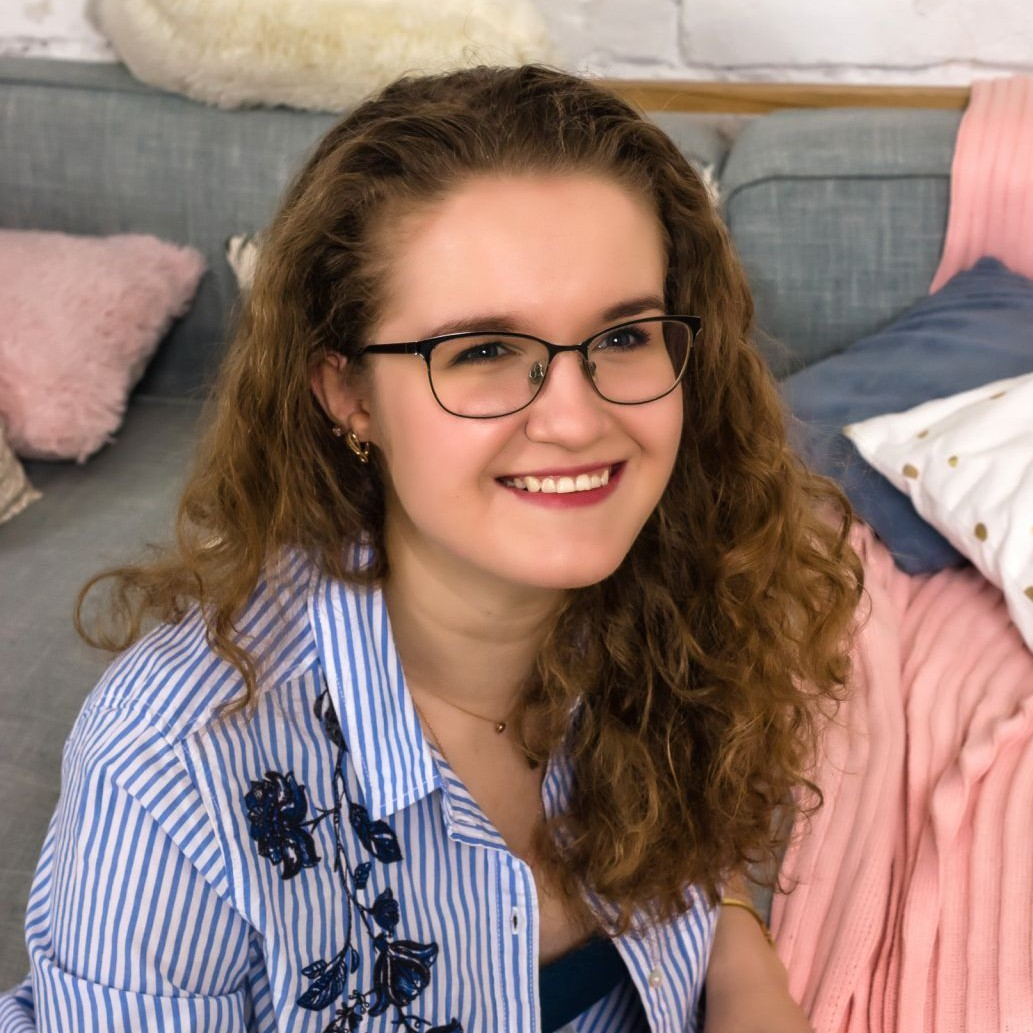
\includegraphics[width=2.8cm]{photo.jpg}
}
\end{tabularx}
\begin{center}
\begin{tabularx}{\linewidth}{@{}*{2}{X}@{}}
% left side %
{
    \csection{EXPERIENCE}{\small
        \begin{itemize}
            \item \frcontent{Holidu GmbH}{Working Student - Munich, Germany}{Backend developer, Java 11 with Spring Boot, running on Kubernetes. Data storage with Elasticsearch 7, PostgreSQL, MongoDB, Redis}{October 2022 - May 2023}
        
            \item \frcontent{RideBee}{Working Student - Munich, Germany}{Native Android application development (Kotlin)}{October 2022 - May 2023}
        
            \item \frcontent{Bao Solutions GmbH}{Working Student - Munich, Germany}{Full stack web development (Vue JS frontend + Python Django backend).}{September 2021 - December 2022}
            
            \item \frcontent{JetBrains}{Software Engineer - Saint-Petersburg, Russia}{Java & Kotlin developer. Was responsible for the maintaining and developing of the Web and mobile applications.}{July 2018 - September 2020}
        \end{itemize}
    }
    
    \csection{EDUCATION}{\small
        \begin{itemize}
            \item \frcontent{Master of Informatics}{Technical University of Munich}{Major study area: Computer Vision. Second study area: Software development.}{2020 - Present}
            \item \frcontent{Bachelor of Applied Mathematics and Information Science}{National Research University Higher School of Economics}{Major study area: Machine Learning. Second study area: Software development. As a part of my bachelor's thesis I developed a platform for reinforcement learning experiments in a 3D graphical environment.}{2019}
        \end{itemize}
    }
    
    

} 
% end left side %
& 
% right side %
{
\csection{PROJECTS}{\small
        \begin{itemize}
            \item \textbf{Android Application on Java} \newline
            {\footnotesize Polyglotte: application for learning words in foreign languages. The app allows storing unknown words with their translations, learning them using the index cards technique, and playing small games to better memorize words.}{}{}
            \item \textbf{iOS Application on Swift} \newline
            {\footnotesize Todoist: a prototype of the task manager application that uses responsive SwiftUI framework.}{}{}
            \item \textbf{Web Application: Java backend + Angular JS frontend} \newline
            {\footnotesize A team project from the "Advanced topics of SE" course at TUM. An online IDE for Java and C++ code.}{}{}
        \end{itemize}
    }
    
    \csection{SD SKILLS}{\small
        \begin{itemize}
            \item \textbf{Programming languages} \newline
            {\footnotesize Java, Kotlin, Swift, Python, JavaScript, SQL, HTML/CSS}{}{}
            \item \textbf{Technologies} \newline
            {\footnotesize Git, Docker, Spring Boot, Gradle, Maven, AWS, Kubernetes}{}{}
        \end{itemize}
    }
    
    \csection{LANGUAGES}{\small
        \begin{itemize}
        \setlength\itemsep{-0.5em}
            \item \textbf{Russian} : Native speaker% \newline
            \item \textbf{English} : C1 %\newline
            \item \textbf{French} : B2 %\newline
            \item \textbf{German} : B2% \newline
        \end{itemize}
    }

}
\end{tabularx}
\end{center}
\end{document}